% Created 2016-11-16 Wed 05:26
\documentclass[11pt]{article}
\usepackage[utf8]{inputenc}
\usepackage[T1]{fontenc}
\usepackage{fixltx2e}
\usepackage{graphicx}
\usepackage{longtable}
\usepackage{float}
\usepackage{wrapfig}
\usepackage{rotating}
\usepackage[normalem]{ulem}
\usepackage{amsmath}
\usepackage{textcomp}
\usepackage{marvosym}
\usepackage{wasysym}
\usepackage{amssymb}
\usepackage{hyperref}
\tolerance=1000
\usepackage[utf8]{inputenc}
\usepackage[spanish, es-noshorthands, es-tabla, english]{babel}
\usepackage{minted}
\usepackage{amsmath}
\usepackage{amssymb}
\usepackage{etoolbox}
\usepackage{xinttools}
\usepackage{graphicx}
\usepackage{lscape}
\usepackage{geometry}
\usemintedstyle{emacs}
\newcommand{\subjectname}{F1005 Electricidad y Magnetismo}
\newcommand{\documenttitle}{Proyecto Final: Simulador de partículas cargadas}
\newcommand{\profesorname}{Profesor Edgar René López Mena}
\newcommand{\authornames}{%
Pablo Muñoz Haro A01222422,%
Andrés Barro Encinas A00226225
}
\input{/Users/home/pablo/latex/templates/org_tec_titlepage}
\author{Pablo Muñoz Haro}
\date{\today}
\title{project}
\hypersetup{
  pdfkeywords={},
  pdfsubject={},
  pdfcreator={Emacs 25.1.1 (Org mode 8.2.10)}}
\begin{document}

\maketitle
\tableofcontents

\clearpage

\section{Introducción}
\label{sec-1}
Este documento contiene el análisis, diseño y documentación de el
proyecto "Simulador de partículas cargadas" desarrollado para la clase
de Electricidad y Magnetismo impartida por el profesor Edgar René en
el Tecnológico de Monterrey Campus Guadalajara para el semestre de
Ago-Dic 2016.

El proyecto consiste de una aplicación que puede ser visistada y
utilizada en un navegador web moderno. La aplicación provee al usuario
con ciertos sistemas de partículas predefinidos, los cuáles pueden ser
modificados en cierta medida y que al momento de presionar "Start" se
comienza a generar una animación que simula la interacción de
partículas cargadas.

\section{Requerimientos}
\label{sec-2}
\begin{itemize}
\item El sistema debe ser accesable a través de un navegador de internet.
\item El sistema debe contener sistemas precargados de partículas que sólo
requieran de pequeñas customizaciones.
\item El sistema debe de incorporar el concepto de "velocidad del tiempo"
que quiere decir que el usuario pueda configurar cuanto representa
un segundo del mundo real en segundos de la simulación.
\item El sistema debe permitir que el usuario seleccione la métrica de
"pixeles por metro" de manera que pueda cambiar la escala de lo que
es capaz de simular y visualizar.
\item Las simulaciones deben correr de manera eficiente, sin
interrupciones ni demoras.
\end{itemize}

\section{Tecnologías utilizadas}
\label{sec-3}
Como cualquier otra página de internet, el proyecto hace uso
significativo de los lenguajes de \emph{HTML} y \emph{CSS} (para la
presentación) y \emph{JavaScript} (para la lógica). En cuanto a este último
también se utilizan las librerías de \emph{PaperJS} para realizar dibujos
en el elemento canvas de HTML, \emph{underscore} para poder aplicar el
paradigma funcional, \emph{Vue} para sincronizar el input del usuario con
los valores de las instancias y \emph{bootstrap} para la interactividad de
la interfaz de usuario.

\section{Control de versiones}
\label{sec-4}
El sistema de control de versiones Git será utilizado mediante el
portal Github. El repositorio con la rama maestra del código puede ser
encontrado en la liga \url{https://github.com/pablo-munoz/proyecto-electro}.

\section{Identificación de entidades}
\label{sec-5}
El sistema contará con entidades que representarán a las
partículas. Cada instancia de estas entidades mantendrá la información
necesaria sobre su estado así como las operaciones que permitirán
dibujarlas, trasladarlas y modificarlas.

A su vez, el sistema contendrá la entidad de "sistemas de carga", los
cuáles estarán compuestos de dos o más instancias de partículas y
estarán encargadas de orquestrar la interacción entre estas.


\newgeometry{a4paper,left=1in,right=1in,top=1in,bottom=1in}
\begin{landscape}
  \section{Diagrama de clases (UML)}
  \begin{figure}[H]
    \centering
    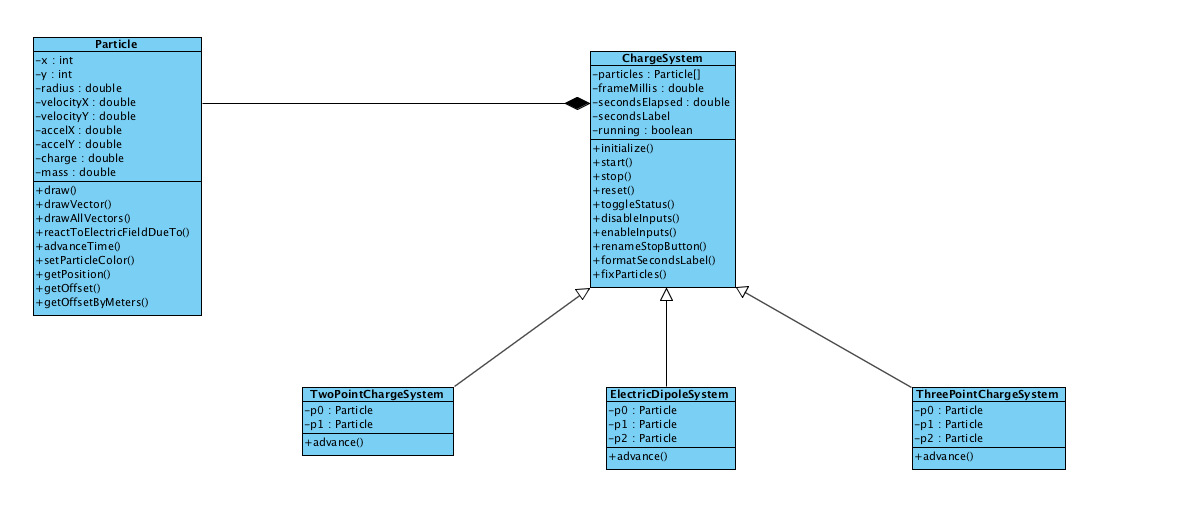
\includegraphics[width=.9\linewidth]{classes-uml.png}
    \caption{Calendario de trabajo}
    \label{fig:calendar}
  \end{figure}
\end{landscape}
\restoregeometry % Restore the global document page margins

\section{Página web}
\label{sec-6}
El programa puede ser accesado a través de la liga:

\url{https://pablo-munoz.github.io/proyecto-electro/index.html}

\section{Física}
\label{sec-7}
\subsection{Ley de Coulomb}
\label{sec-7-1}
La ley de Coulomb define como es que cargas puntuales interactúan
entre sí. Esto incluye cuando las cargas se atraen o repelen. En este
proyecto la fuerza elécctrica es calculada utilizando la ecuación de
esta ley.

Debido a que la representación interna de las partículas guarda la
coordenada $x$ y $y$, el cálculo interno de las fuerzas también se
desglosa en components $x$ y $y$.

\begin{align*}
  F_x = \cos ( \theta ) \frac{1}{4 \pi \epsilon_0} \frac{\vert q_1 q_2 \vert}{r^2} =
  \frac{x}{\sqrt{x^2 + y^2}} \frac{1}{4 \pi \epsilon_0} \frac{\vert q_1 q_2 \vert}{ (\sqrt{x^2 + y^2 })^2 } =
  \frac{x \vert q_1 q_2 \vert }{4 \pi \epsilon_0 (x^2 + y^2)^{\frac{3}{2}}} \\
  F_y = \sin ( \theta ) \frac{1}{4 \pi \epsilon_0} \frac{\vert q_1 q_2 \vert}{r^2} =
  \frac{y}{\sqrt{x^2 + y^2}} \frac{1}{4 \pi \epsilon_0} \frac{\vert q_1 q_2 \vert}{ (\sqrt{x^2 + y^2 })^2 } =
  \frac{y \vert q_1 q_2 \vert }{4 \pi \epsilon_0 (x^2 + y^2)^{\frac{3}{2}}}
\end{align*}

\subsection{Dipolo Eléctrico}
\label{sec-7-2}
Un dipolo eléctrico es un Sistema formado por dos cargas separadas por
una distancia. Las magnitudes de las cargas deben ser iguales y los
signos opuestos.

Modificando los valores desde la interfaz gráfica, es posible crear un
dipolo y observar los valores de las distintas magnitudes para cada
una de las cargas individuales. 

Si se comienza la simulación, se puede observar una representación
aproximada de su comportamiento.

\subsection{Energía potencial eléctrica}
\label{sec-7-3}
Para cada partícula, se puede obtener una energía potencial con
respecto del resto de las partículas. Cada una de las partículas del
sistema calculara su energía potencial de manera individual. 

Para calcular se utiliza la formula sin modificaciones ya que esta no
cuenta con componentes x o y, es solo una magnitud.


\section{Código Fuente}
\label{sec-8}
\subsection{\texttt{HTML}}
\label{sec-8-1}
\begin{minted}[frame=lines,fontsize=\footnotesize,breaklines,linenos]{html}
<html>
    <head>
        <script
            src="https://code.jquery.com/jquery-3.1.1.min.js"
            integrity="sha256-hVVnYaiADRTO2PzUGmuLJr8BLUSjGIZsDYGmIJLv2b8="
            crossorigin="anonymous"></script>
        <!-- Latest compiled and minified CSS -->
        <link rel="stylesheet" href="https://maxcdn.bootstrapcdn.com/bootstrap/3.3.7/css/bootstrap.min.css"
              integrity="sha384-BVYiiSIFeK1dGmJRAkycuHAHRg32OmUcww7on3RYdg4Va+PmSTsz/K68vbdEjh4u" crossorigin="anonymous">
        <!-- Latest compiled and minified JavaScript -->
        <script src="https://maxcdn.bootstrapcdn.com/bootstrap/3.3.7/js/bootstrap.min.js"
                integrity="sha384-Tc5IQib027qvyjSMfHjOMaLkfuWVxZxUPnCJA7l2mCWNIpG9mGCD8wGNIcPD7Txa" crossorigin="anonymous"></script>
        <script src="https://cdn.jsdelivr.net/lodash/4.16.3/lodash.min.js"></script>
        <script src="https://cdnjs.cloudflare.com/ajax/libs/paper.js/0.10.2/paper-full.js" type="text/javascript"></script>
        <script src="https://unpkg.com/vue/dist/vue.js"></script>
        <script src="projectv2.js" type="text/javascript"></script>
        <style type="text/css">
         body {
             background: url('grey.png') repeat;
         }

         canvas {
             border: 1px solid #ccc;
             background-color: white;
         }

         .particle-controls {
             background-color: #fff;
         }

         .unselectable {
             -webkit-user-select: none; /* Chrome/Safari */        
             -moz-user-select: none; /* Firefox */
             -ms-user-select: none; /* IE10+ */
             /* Rules below not implemented in browsers yet */
             -o-user-select: none;
             user-select: none;
             cursor: pointer;
         }
        </style>
    </head>
    <body>
        <div class="container" style="margin-top: 50">
            <div class="col-md-8" id="canvas-container">
                <canvas id="canvas" width="970" height="920"></canvas>
            </div>
            <div id="app" class="controls">
                <div class="col-md-4">
                    <div class="form-group">
                        <select id="charge-system-selector" class="form-control" v-on:change="changeChargeSystem()">
                            <option value="twoChargeSystem">Two charge system</option>
                            <option value="threeChargeSystem">Three charge system</option>
                            <option value="electricDipole">Two Static Charges</option>
                        </select>
                    </div>
                    <div class="form-group">
                        <div class="input-group">
                            <input class="form-control ppm" type="text" type="number" v-bind:value="pixelsPerMeter" v-on:change="updatePixelsPerMeter()" type="number"/>
                            <span class="input-group-addon">piexels per meter.</span>
                        </div>
                    </div>
                    <div class="form-group">
                        <div class="input-group">
                            <span class="input-group-addon">1 real second =</span>
                            <input class="form-control" type="text" v-model="simulation.frameMillis" type="number" v-on:change/>
                            <span class="input-group-addon">simul seconds.</span>
                        </div>
                    </div>
                    <button id="start-stop-btn" class="btn btn-primary" onClick="simulation.toggleStatus();">Start</button>
                    <button id="reset-btn" class="btn btn-danger" onClick="simulation.reset();">Reset</button>

                    <div class="particle-controls" v-for="(particle, index) in simulation.particles">
                        <particle-controls
                            :particle="particle"
                            :index="index"/>
                    </div>

                </div>
            </div>
        </div>
    </body>
</html>
\end{minted}

\subsection{\texttt{Manifest constants}}
\label{sec-8-2}
\begin{minted}[frame=lines,fontsize=\footnotesize,breaklines,linenos]{javascript}
paper.install(window);

var WINDOW_WIDTH  = 970;
var WINDOW_HEIGHT = 720;

const PERMITIVITY     = 9 * Math.pow(10, 9);
const ELECTRON_CHARGE = -1.602 * Math.pow(10, -19);
const PROTON_CHARGE   = -ELECTRON_CHARGE;
const PROTON_MASS     = 1.6727 * Math.pow(10, -27);
const NEUTRON_MASS    = 1.6750 * Math.pow(10, -27);
const ELECTRON_MASS   =  9.110 * Math.pow(10, -31);
const VECTOR_WIDTH = 2;
\end{minted}

\subsection{\texttt{Globals}}
\label{sec-8-3}
\begin{minted}[frame=lines,fontsize=\footnotesize,breaklines,linenos]{javascript}
var PIXELS_PER_METER = 100;
var simulation = undefined;
var app = undefined;
\end{minted}

\subsection{\texttt{class Particle}}
\label{sec-8-4}
\begin{minted}[frame=lines,fontsize=\footnotesize,breaklines,linenos]{javascript}
class Particle {
    // x, y, radius
    constructor(args) {
        _.assign(this, _.defaults(args, {
            x: 0,
            y: 0,
            radius: 8,
            velocityX: 0,            // m/s
            velocityY: 0,            // m/s
            accelX: 0,               // m/s
            accelY: 0,               // m/s
            charge: ELECTRON_CHARGE, // C
            mass: ELECTRON_MASS      // kg
        }));
        this.forceX = 0;
        this.forceY = 0;
        this.potentialEnergy = 0;
    }

    draw() {
        this.forceVector = new Path.Line(new Point(this.x, this.y), new Point(this.x, this.y));
        this.forceVector.strokeWidth = VECTOR_WIDTH;
        this.forceVector.strokeColor = 'rgba(255, 255, 255, 0.5)';
        this.accelVector = new Path.Line(new Point(this.x, this.y), new Point(this.x, this.y));
        this.accelVector.strokeWidth = VECTOR_WIDTH;
        this.accelVector.strokeColor = 'rgba(255, 0, 0, 0.5)';
        this.velocityVector = new Path.Line(new Point(this.x, this.y), new Point(this.x, this.y));
        this.velocityVector.strokeWidth = VECTOR_WIDTH;
        this.velocityVector.strokeColor = 'rgba(0, 255, 0, 0.5)';
        this.circle = new Path.Circle(new Point(this.x * PIXELS_PER_METER + WINDOW_WIDTH/2, -this.y * PIXELS_PER_METER + WINDOW_HEIGHT/2), this.radius);
        this.label = new PointText(this.x * PIXELS_PER_METER + WINDOW_WIDTH/2 - 2, -this.y * PIXELS_PER_METER + WINDOW_HEIGHT/2 + 2);
        this.label.strokeColor = 'white';
        this.label.content = this.name;
        this.label.fontSize = 8;
        this.circle.onMouseDrag = this.label.onMouseDrag = _.bind(function(event) {
            this.circle.translate(event.delta);
            this.label.translate(event.delta);
            this.x = (this.circle.position.x - WINDOW_WIDTH/2) / PIXELS_PER_METER;
            this.y = -(this.circle.position.y - WINDOW_HEIGHT/2) / PIXELS_PER_METER;
            this.drawAllVectors();
        }, this);
        this.setParticleColor();
    }

    drawVector(whichVector) {
        this[whichVector + 'Vector'].segments = [this.getPosition(), this.getOffsetByMeters(new Point(this[whichVector + 'X'] * PIXELS_PER_METER, -this[whichVector + 'Y'] * PIXELS_PER_METER))];
    }

    drawAllVectors() {
        _.forEach(['force', 'velocity', 'accel'], _.bind(function(whichVector) {
            this.drawVector(whichVector);
        }, this));
    }

    reactToElectricFieldDueTo(otherParticleList) {
        this.forceX = this.forceY = this.accelX = this.accelY = this.potentialEnergy = 0;

        _.forEach(otherParticleList, _.bind(function(otherParticle) {
            const distanceX = (this.x - otherParticle.x);
            const distanceY = (this.y - otherParticle.y);
            if((distanceX == 0 && distanceY == 0) || this === otherParticle) {
                return;
            }
            const qq = (this.charge * otherParticle.charge);
            const auxiliarForce = PERMITIVITY * ( ( qq ) / Math.pow(( distanceX * distanceX + distanceY * distanceY), 3/2) );
            this.potentialEnergy += auxiliarForce * ( distanceX * distanceX + distanceY * distanceY);
            this.forceX += distanceX * auxiliarForce;
            this.forceY += distanceY * auxiliarForce;
        }, this));
        this.accelX = this.forceX / this.mass;
        this.accelY = this.forceY / this.mass;
    }

    advanceTime(milliseconds) {
        const seconds = milliseconds / 1000;
        this.velocityX += this.accelX * seconds;
        this.velocityY += this.accelY * seconds;
        this.x += this.velocityX * seconds;
        this.y += this.velocityY * seconds;
        var translatePoint = new Point(this.velocityX * seconds * PIXELS_PER_METER, -1 * this.velocityY * seconds * PIXELS_PER_METER);
        this.circle.translate(translatePoint);
        this.label.translate(translatePoint);
        this.drawAllVectors();
    }

    setParticleColor() {
        if (this.charge > 0) {
            this.circle.fillColor = 'red';
        } else if (this.charge < 0) {
            this.circle.fillColor = 'blue';
        }
    }

    getPosition() {
        return new Point(this.circle.position.x, this.circle.position.y);
    }

    getOffset(offsetPoint) {
        return this.getPosition().add(offsetPoint);
    }

    getOffsetByMeters(offsetPointMeters) {
        return this.getOffset(offsetPointMeters.multiply(PIXELS_PER_METER));
    }

}
\end{minted}

\subsection{\texttt{class ChargeSystem}}
\label{sec-8-5}
\begin{minted}[frame=lines,fontsize=\footnotesize,breaklines,linenos]{javascript}
class ChargeSystem {
    constructor() {
        this.initialize();
        this.running = false;
    }

    initialize() {
        paper.project.activeLayer.removeChildren();
        this.particles = [];
        this.frameMillis = 1000/60;
        this.secondsElapsed = 0;

        this.secondsLabel = new PointText(20, 20);
        this.secondsLabel.fontSize = 16;
        this.formatSecondsLabel();
    }

    start() {
        this.refreshIntervalId = setInterval(_.bind(function() {
            this.advance();
            this.formatSecondsLabel();
            this.secondsElapsed += this.frameMillis / 1000;
        }, this), 1000/60/*this.frameMillis*/);
        this.disableInputs();
        this.running = true;
        this.renameStartStopButton();
    }

    stop() {
        clearInterval(this.refreshIntervalId);
        this.running = false;
        this.renameStartStopButton();
    }

    reset() {
        PIXELS_PER_METER = 100;
        app.$set(app, 'pixelsPerMeter', 100);
        this.secondsElapsed = 0;
        clearInterval(this.refreshIntervalId);
        this.refreshIntervalId = undefined;
        this.initialize();
        this.running = false;
        this.enableInputs();
        this.renameStartStopButton();
    }

    toggleStatus() {
        if (!this.running) {
            this.start();
        } else {
            this.stop();
        }
    }

    disableInputs() {
        $('input').attr('disabled', 'disabled');
    }

    enableInputs() {
        $('input').attr('disabled', null);
    }

    renameStartStopButton() {
        if (this.running) {
            $('#start-stop-btn').text('Stop');
        } else {
            $('#start-stop-btn').text('Start');
        }
    }

    formatSecondsLabel() {
        this.secondsLabel.content = "t = " + this.secondsElapsed + "s";
    }

    fixParticles(){
        _.forEach(this.particles, _.bind(function(particle) {
            particle.x = (particle.circle.position.x - WINDOW_WIDTH/2) / PIXELS_PER_METER;
            particle.y = -(particle.circle.position.y - WINDOW_HEIGHT/2) / PIXELS_PER_METER;
        }, this));
    }
}
\end{minted}

\subsection{\texttt{class TwoChargeSystem}}
\label{sec-8-6}
\begin{minted}[frame=lines,fontsize=\footnotesize,breaklines,linenos]{javascript}
class TwoPointChargeSystem extends ChargeSystem {
    initialize() {
        super.initialize();
        this.p0 = new Particle({
            x: 3,
            velocityX: 0,
            velocityY: -5,
            charge: ELECTRON_CHARGE,
            mass: ELECTRON_MASS,
            name: '0'
        });
        this.particles.push(this.p0);
        this.p0.draw();

        this.p1 = new Particle({
            x: 0,
            velocityX: 0,
            velocityY: 0,
            charge: PROTON_CHARGE,
            mass: PROTON_MASS,
            name: '1'
        });
        this.particles.push(this.p1);
        this.p1.draw();
    }

    advance() {
        _.forEach(this.particles, _.bind(function(particle) {
            particle.reactToElectricFieldDueTo(this.particles);
        }, this));
        _.forEach(this.particles, _.bind(function(particle) {
            particle.advanceTime(this.frameMillis);
        }, this));
    }
}
\end{minted}

\subsection{\texttt{class ElectricDipole}}
\label{sec-8-7}
\begin{minted}[frame=lines,fontsize=\footnotesize,breaklines,linenos]{javascript}
class ElectricDipoleSystem extends ChargeSystem {
    initialize() {
        // p1 and p1 are the "fixed" ones
        super.initialize();
        this.p0 = new Particle({
            x: 2,
            y: 0,
            charge: ELECTRON_CHARGE,
            mass: ELECTRON_MASS,
            name: '0'
        });
        this.particles.push(this.p0);
        this.p0.draw();

        this.p1 = new Particle({
            y: -1,
            charge: ELECTRON_CHARGE,
            mass: ELECTRON_MASS,
            name: '1'
        });
        this.particles.push(this.p1);
        this.p1.draw();

        this.p2 = new Particle({
            y: 1,
            charge: this.p1.charge,
            mass: this.p1.mass,
            name: '2'
        });
        this.particles.push(this.p2);
        this.p2.draw();
    }

    advance() {
        this.p0.reactToElectricFieldDueTo(this.particles);
        this.p0.advanceTime(this.frameMillis);
    }
}
\end{minted}

\subsection{\texttt{class ThreeChargeSystem}}
\label{sec-8-8}
\begin{minted}[frame=lines,fontsize=\footnotesize,breaklines,linenos]{javascript}
class ThreePointChargeSystem extends ChargeSystem {
    initialize() {
        super.initialize();
        this.p0 = new Particle({
            x: 3,
            velocityX: 0,
            velocityY: 5,
            charge: ELECTRON_CHARGE,
            mass: ELECTRON_MASS,
            name: '0'
        });
        this.particles.push(this.p0);
        this.p0.draw();

        this.p1 = new Particle({
            x: 0,
            velocityX: 0,
            velocityY: 0,
            charge: PROTON_CHARGE,
            mass: PROTON_MASS,
            name: '1'
        });
        this.particles.push(this.p1);
        this.p1.draw();

        this.p2 = new Particle({
            x: -3,
            velocityX: 0,
            velocityY: -5,
            charge: ELECTRON_CHARGE,
            mass: ELECTRON_MASS,
            name: '2'
        });
        this.particles.push(this.p2);
        this.p2.draw();

        _.forEach(this.particles, _.bind(function(particle) {
            particle.reactToElectricFieldDueTo(this.particles);
        }, this));
    }

    advance() {
        _.forEach(this.particles, _.bind(function(particle) {
            particle.reactToElectricFieldDueTo(this.particles);
        }, this));
        _.forEach(this.particles, _.bind(function(particle) {
            particle.advanceTime(this.frameMillis);
        }, this));
    }
}
\end{minted}
\subsection{\texttt{onload script}}
\label{sec-8-9}
\begin{minted}[frame=lines,fontsize=\footnotesize,breaklines,linenos]{java}
window.onload = function() {
    $('#canvas').width($('#canvas-container').width());

    WINDOW_WIDTH  = $('#canvas-container').width();
    WINDOW_HEIGHT = $('#canvas-container').height();

    paper.setup('canvas');

    simulation = new TwoPointChargeSystem();

    app = new Vue({
        el: '#app',
        data: {
            pixelsPerMeter: PIXELS_PER_METER,
            updatePixelsPerMeter: function(event) {
                var newValue = $('input.ppm').val();
                PIXELS_PER_METER = newValue;
                app.pixelsPerMeter = newValue;
                simulation.fixParticles();
            },
            simulation: simulation,
            changeChargeSystem: function() {
                var selectedSystem = $('#charge-system-selector').val();
                simulation.reset();
                app.simulation = simulation = new SYSTEMS_MAP[selectedSystem]();
            }
        },
        components: {
            "particle-controls": {
                props: ['index', 'particle'],
                data: function() {
                    return {
                        showing: true
                    };
                },
                template: `
<div class="panel panel-warning">
    <div class="panel-heading unselectable" v-on:click="showing = !showing">
        <span>Particle {{ index }}</span>
        <span class="glyphicon glyphicon-chevron-down pull-right" v-show="!showing"></span>
        <span class="glyphicon glyphicon-chevron-up pull-right" v-show="showing"></span>
    </div>
    <div class="panel-body" v-show="showing">
        <div class="form-group">
            <div class="input-group">
                <span class="input-group-addon">q =</span>
                <input class="form-control" type="number" v-model="particle.charge" v-on:change="particle.setParticleColor()"/>
                <span class="input-group-addon">C</span>
            </div>
        </div>
        <div class="form-group">
            <div class="input-group">
                <span class="input-group-addon">m =</span>
                <input class="form-control" type="number" v-model="particle.mass"/>
                <span class="input-group-addon">kg</span>
            </div>
        </div>
        <div class="form-group">
            <div class="input-group">
                <span class="input-group-addon">vx =</span>
                <input class="form-control" type="number" v-model="particle.velocityX"/>
                <span class="input-group-addon">m/s</span>
            </div>
        </div>
        <div class="form-group">
            <div class="input-group">
                <span class="input-group-addon">ax =</span>
                <input class="form-control" type="number" v-model="particle.accelX"/>
                <span class="input-group-addon">m/s^2</span>
            </div>
        </div>
        <div class="form-group">
            <div class="input-group">
                <span class="input-group-addon">vy =</span>
                <input class="form-control" type="number" v-model="particle.velocityY"/>
                <span class="input-group-addon">m/s</span>
            </div>
        </div>
        <div class="form-group">
            <div class="input-group">
                <span class="input-group-addon">ay =</span>
                <input class="form-control" type="number" v-model="particle.accelY"/>
                <span class="input-group-addon">m/s^2</span>
            </div>
        </div>
    </div>
</div>
`
            }
        }
    });
}
\end{minted}
\section{Capturas de pantalla del programa en funcionamiento}
\label{sec-9}
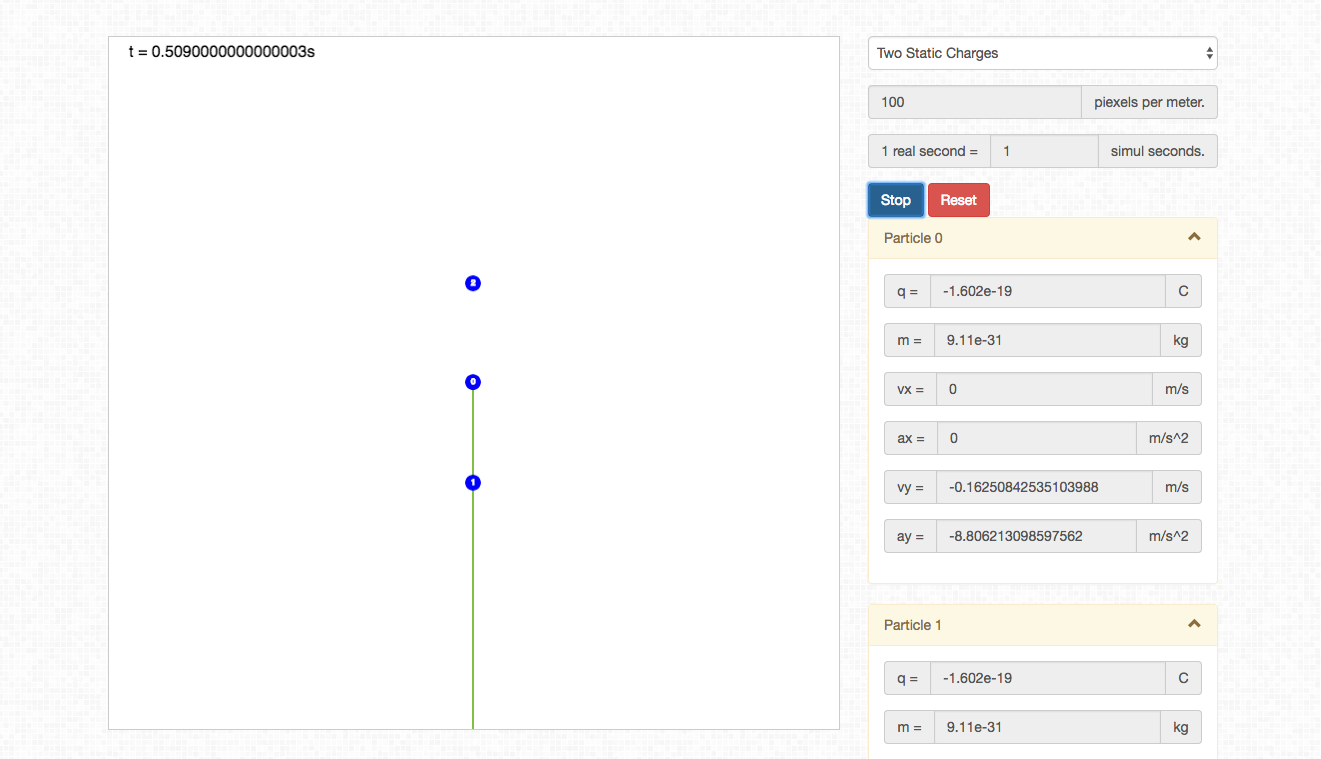
\includegraphics[width=\linewidth]{sc1.png}
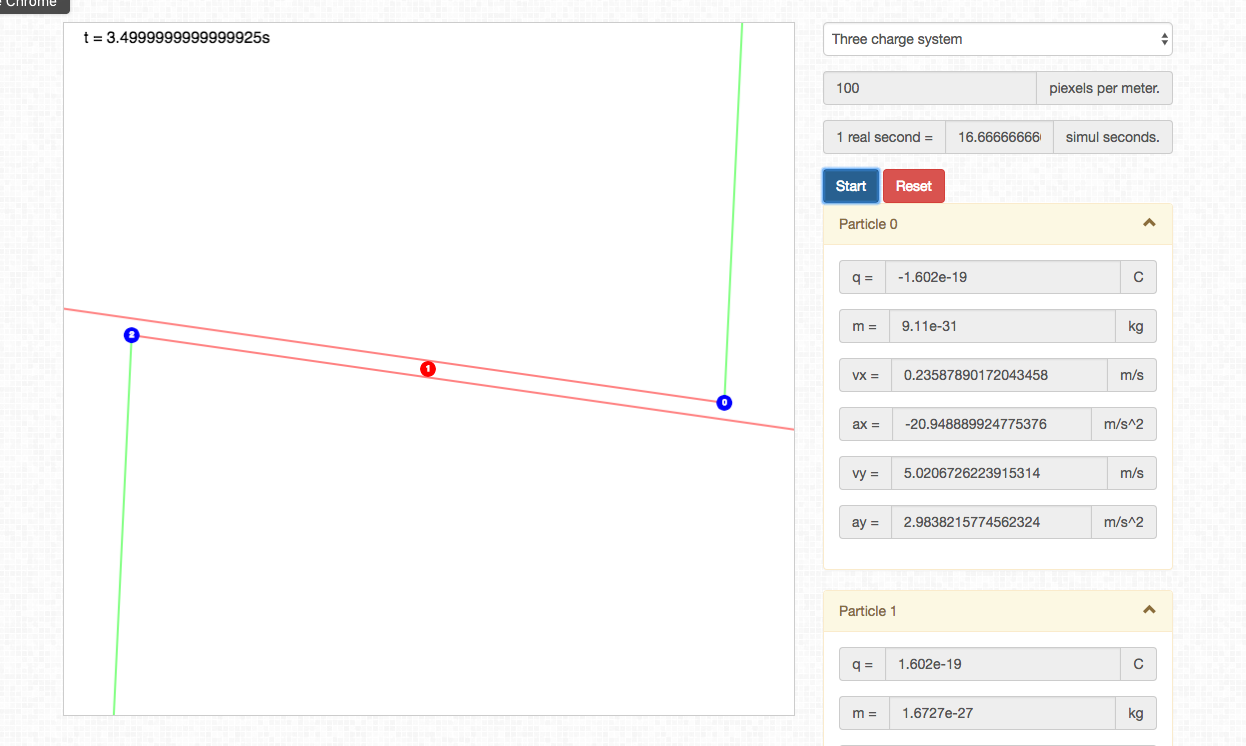
\includegraphics[width=\linewidth]{sc2.png}
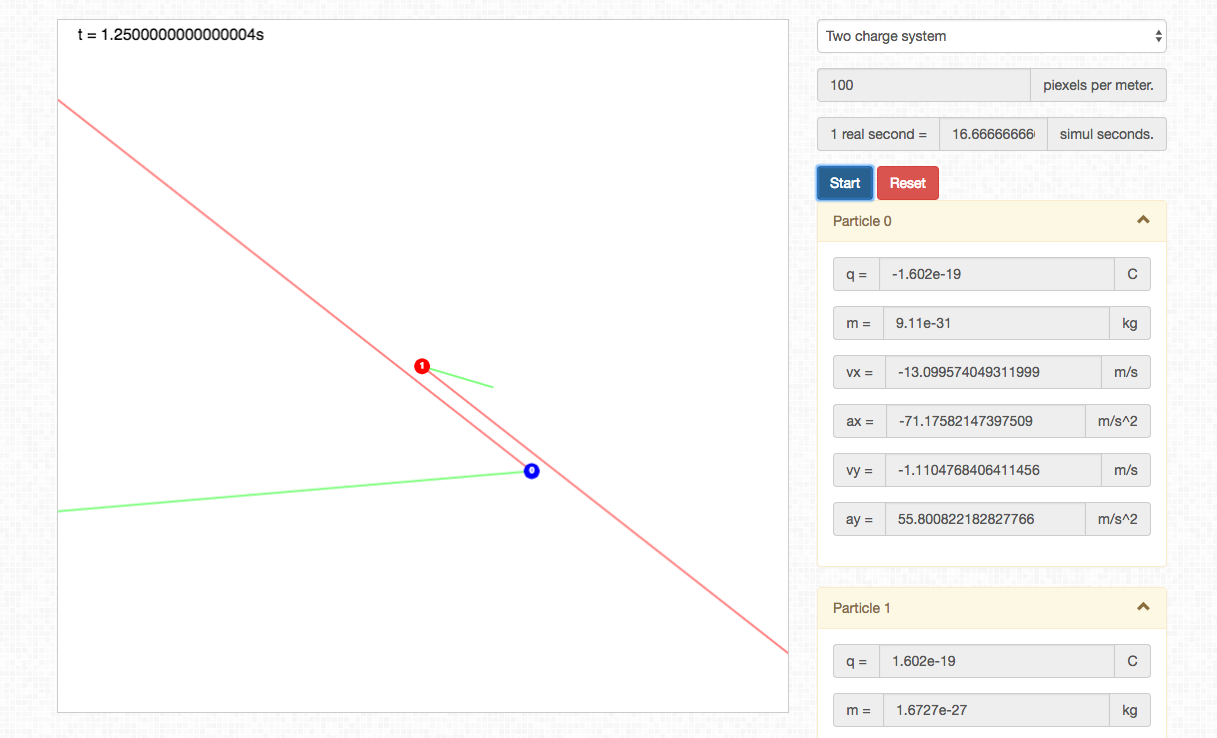
\includegraphics[width=\linewidth]{sc3.png}
% Emacs 25.1.1 (Org mode 8.2.10)
\end{document}